\documentclass{school-22.211-notes}
\date{March 14, 2012}

\begin{document}
\maketitle

%%%%%%%%%%%%%%%%%%%%%%%%%%%% Exam 1 Review Begin %%%%%%%%%%%%%%%%%%%%%%%%%%%%%%%%%%%%%%%%%%
\lecture{Exam 1 Review}
\topic{Most Important Concepts}
\begin{enumerate}
\item Basic Nuclear Data: know 1.0 kT correspond to 0.0253 eV. Know number density 
  \eqn{ N = \frac{\rho N_A}{M} }
  where $N_A$ is  avogado's number, take $0.6022$, $\rho$ is density in g/cc, $M$ is atomic mass (unitless). 

\item Four pieces of nuclear physics: 
  \begin{enumerate}
    \item Fission Spectra    
      \begin{enumerate}
      \item A hump in high energy. Reason: fission spectrum, degraded due to scattering; 
      \item A slight decrease in the epithermal region. Reason: resonant capture losses, esp. U238; 
      \item A hump in low energy. Reason: Maxwell distribution of the thermal agitation but a little harder because the temperature equilibrium has not been perfectly achieved. 
      \end{enumerate}

    \item Elastic Scattering
      \begin{enumerate}
      \item Asymptotic elastic scattering for high energy (above 4eV): assume isotropic scattering in COM. Generate $1/E$ spectrum; asymptotic flux value is $\Phi_{as} (u) = \frac{S}{\xi \Sigma_s (u)}$ according to Reuss (7.2.3). 
      \item Thermal elastic scattering (below 4eV): use elastic scattering for monatomic (Maxwellian) free gas; may up-scatter. 
      \item  \textbf{Spring 2012 Exam 1 \#11, \#12:} for a neutron asymptotically elastic scattering off hydrogen, the probability density function is flat: 
        \eqn{ p(E'\to E) = \frac{1}{E'} }
        Then the probability of the next collision happening within $[E_1,E_2]$ is, 
        \eqn{ \int_{E_1}^{E_2} \frac{1}{E'} \dE }
      \end{enumerate}

    \item SLBW Resonance: the SLBW scattering cross section is, 
      \eqn{ \sigma_s (x) &= \frac{2}{\Gamma} (r \psi(x) + q \chi(x)) + \sigma_p}
      where 
      \eqn{ x &= \frac{2(E -E_0)}{\Gamma} &\psi &= \frac{1}{1+x^2} &\chi&= \frac{2x}{1+x^2} }
      \textbf{Spring 2012 Exam 1 \#6:} given $r,q, \Gamma,T$, at what energy does the scattering cross section peak? 
      \begin{itemize}
        \item Solve for $\frac{\dsigma_s}{\dx} = 0$ for $x$, then plug into the definition for $x$ for $E$.
        \item Alternatively, in this problem $r \ll q$, $\chi$ dominate the scattering cross section, and $\chi$ maximize at $x=1$, hence $x=1$. 
      \end{itemize}

    \item Scattering Kernals: 
      \begin{enumerate}
      \item Simple bound thermal scattering: 
      \eqn{ \sigma_{\mbox{bound}} = \left( 1 + \frac{1}{A_{\mathrm{atom}}} \right) \sigma_{\mathrm{free}} }
      \item \textbf{Spring 2012 Exam 1 \#8:} given a thermal scattering kernel whose downscatter or upscatter are symmetric about 1, the probability of up-scattering is 0.5. 
      \item \textbf{Spring 2012 Exam 1 \#9:} for the cdf of the scattering kernel, the $E_{out}/E_{in}$ is the x-axis; that is, the absolute magnitudes of $E_{in}, E_{out}$ do not matter, it is their ratio that matters. 
      \item \textbf{Spring 2012 Exam 1 \#10:} the higher the temperature (for instance, temperature $\gg 1$ kT), the more closely the scattering probability curve follows a box. 
      \end{enumerate}
  \end{enumerate}

\item Homogeneous resonance self-sheilding
  \begin{enumerate}
    \item Infinite media: In infinite medium, the flux shape near resonance depends only on the ratio of the number density of the moderator to the resonance absorber and the moderator cross section. The absolute numbers are not needed until we move into a finite medium and start to worry about leakage. \textbf{2012 Spring Exam 1, \#14}, the infinite dilute microscopic absorption cross section is (similarly any infinitely dilute group cross section), 
      \eqn{ \expect{\sigma} &= \frac{\int_{E_1}^{E_2} \sigma(E) \phi(E) \dE}{\int_{E_1}^{E_2} \phi(E) \dE} = \frac{\int_{E_1}^{E_2} \sigma(E) \frac{1}{E} \dE}{\int_{E_1}^{E_2} \frac{1}{E}  \dE} = \frac{RI}{\ln\left(\frac{E_2}{E_1} \right)} }

    \item Dilution factors: dilution cross section, 
      \eqn{ \sigma_d = \frac{N_m \sigma_m}{N_r} }



    \item Resonance Integral
      \begin{enumerate}
      \item Calculation, \textbf{2012 Spring Exam 1, \#13,\#15}
        \eqn{ \RIeff = - \int_{u1}^{u2} \sigma(u) \du = \int_{E_1}^{E_2} \sigma(E) \frac{1}{E} \dE = \sigma \ln \left( \frac{E_2}{E_1} \right) }
        where $\sigma$ is the resonance xs, not including potential xs. If there are multiple resonances, add them up. 

      \item RI represents the average absorption xs characterizing the resonance, averaged over the flux within the resonance. It is sort of like the averaged reaction rate, or collision density. 
        
      \item Relating to $\sigma_g, \sigma_d$: 
        \eqn{ \RIeff &= \sigma_g \ln{\frac{E_2}{E_1}}  & \RIeff^{u1\to u2} &= \int_{u1}^{u2} \sigma_a^R (u) \frac{\sigma_d}{\sigma_a^R(u) + \sigma_d} \du  }

      \item As temperature increases, $\RIeff$ increases becasue the broadened resonance increases the energy range over which abosprtion occurs. There is less flux depression, whereas the area under the cross section is about the same, result in an increase in the $\RIeff$. \textbf{Spring 2012 Exam 1 \#16:} the infinite dilute RI is independent of temperature because in Doppler broadening the area under the resonance is constant. 

      \item As U/H increases, $\RIeff$ decreases because of energy self-shielding: as U/H increases, more and more self-shielding, the flux is more depressed, result in smaller $\RIeff$. A second consequence is that the higher energy range becomes more important. See Section~\ref{spectral-hardening-section}. 

      \item Narrow resonance $\RIeff$ approximation: assume any scattering with the resonant material scatters neutrons below the resonance energy. 
        \textbf{Spring 2012 Exam 1 \#18}, assuming $1/E$ spectrum, homogeneous mixture of a scattering material and a resonance absorpting material. 
        \eqn{ \RI_{NR} = \int_{E_1}^{E_2} \sigma_r (E) \frac{\sigma_{pr} + \sigma_d}{\sigma_r(E) + \sigma_{pr} + \sigma_d} \frac{1}{E} \dE = \sigma_r \frac{\sigma_{pr} + \sigma_d}{\sigma_r + \sigma_{pr} + \sigma_d} \ln \left(\frac{E_2}{E_1} \right) }        
        where the \uline{background/dilution cross section} for a homogeneous system is (where the underscript $m$ most likely means scattering), 
        \eqn{ \sigma_d = \frac{N_m}{N_r} \sigma_m  }
        
      \item Wide resonance $\RIeff$ approximation: assume scattering with the resonance material leaves the neutron within the resonance energy and they will be absorbed. \textbf{Spring 2012 Exam 1 \#19}.
        \eqn{ \RI_{WR} = \int_{E_1}^{E_2} \sigma_r (E) \frac{\sigma_d}{\sigma_r(E) + \sigma_d} \frac{1}{E} \dE = \sigma_r \frac{ \sigma_d}{\sigma_r +  \sigma_d} \ln \left(\frac{E_2}{E_1} \right) }  
      \end{enumerate}
  \end{enumerate}

\item Doppler effects
  \begin{enumerate}
    \item Psi/chi functions
      \begin{figure}
        \centering
        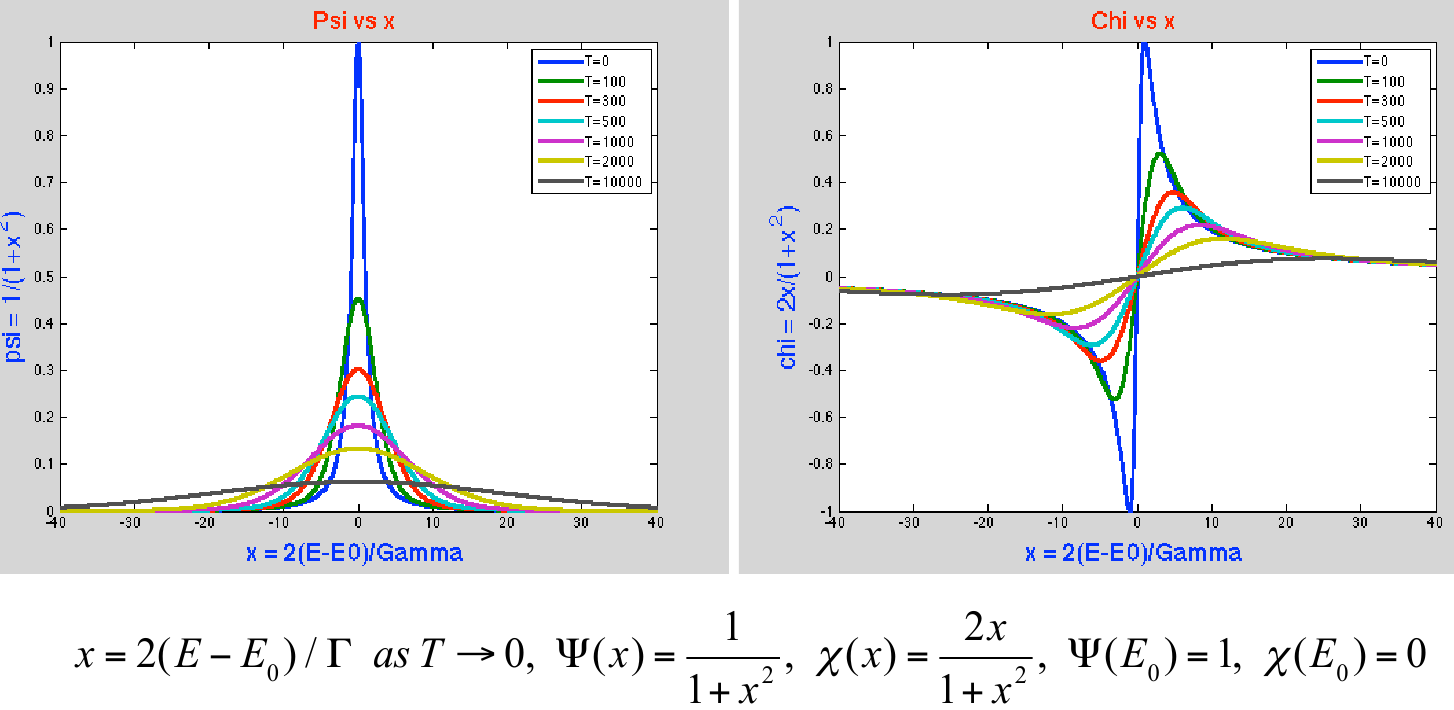
\includegraphics[width=6in]{images/r-m/psi-chi-plot.png}
      \end{figure}

    \item Finite dilution
    \item Temperature effects
  \end{enumerate}

\item Monte Carlo
  \begin{enumerate}
    \item Physical process:  see Table~\ref{plot-MC}
    \item Collision estimators: \textbf{Spring 2012 Exam 1 \#22:}  \ce{U^{238}} absorption  rate per atom, absorption rate is, respectively, 
      \eqn{ &\Sum \frac{\sigma_a^{238}}{\Sigma_t} & N^{238} \Sum \frac{\sigma_a^{238}}{\Sigma_t} & }
    \item Simple statistics:  need enough to provide resolution, but not too many that each bin does not get enough particles.
  \end{enumerate}
  
\item Heterogeneous Self-shielding: see Section~\ref{heterogeneous-geo}.
  \begin{enumerate}
    \item Homogeneous/heterogeneous equivalence: 
      \begin{align*}
        \mbox{Homogeneous mixture energy shape of flux } \phi(u) &= \frac{\sigma_{pot, f} + \sigma_d}{\sigma_{r,f} (u) + \sigma_{pot, f} + \sigma_d}   & \sigma_d &= \frac{N_m \sigma_m}{N_r}  \\
        \mbox{Heterogeneous energy shape of flux in the fuel } \phi_f(u) &= \frac{\sigma_{pot, f} + \sigma_e}{\sigma_{r,f} (u) + \sigma_{pot, f} + \sigma_e}   & \sigma_e &= \frac{S_f}{4 V_f N_r} 
      \end{align*}

    \item Escape probabilities $p$: only depends on effective RI and dilution xs: 
      \eqn{ p \approx \exp \left( - \frac{\RI_{\eff}}{\zeta \sigma_d} \right) = \exp \left( - \frac{N_r \RI_{\eff}}{\zeta \Sigma_m} \right)  }
      Escape cross section $\sigma_e$: 
      \eqn{ \sigma_e = \frac{1}{l N_f} = \frac{S}{4V N_f} }
      \textbf{Spring 2012 Exam 1 \#17:} what is the resonance escape probability for infinitely dilute material 1 in 1 gm/cc material 2? 
      \begin{itemize}
        \item Material 1 is infinitely dilute, so we assume the flux is shaped entirely by material 2 and hence is not affected by the resonances. $p = 1$. 
      \end{itemize}

    \item Collision probabilities 

    \item 2-region reciprocity relation:
      \eqn{ P_{1\to 2} \Sigma_1 V_1 = P_{2\to 1} \Sigma_2 V_2 }


    \item Wigner's rational models, with Bell's refinment and Dancoff correction factor, 
      \eqn{ P_{f\to f}  = \frac{\sigma_{t,f} (u)}{\frac{(1-C)b}{(1-C) + Cb} \sigma_e + \sigma_{t,f} (u)}  } 
      where Dancoff factor is approximated from slide 28 Lec7, escape cross section is calculated for a cylinder to be $\Sigma_e = \frac{1}{2r}$.  Upon getting $P_{ff}$, we find $P_{fm} = 1 - P_{ff}$, then use reciprocity to find $P_{mf}$. See \textbf{Spring 2012 Exam 1: \#20}. 

    \item Dancoff factors


    \item $1/E$ fluxes: true except when resonant absorber is present (recall we keep using 1/E for spectrum above the resonance). 
  \begin{itemize}
  \item It is characteristic of the scalar flux in the slowing down energy range, as long as there is no up-scattering and no fission source. 
  \item It arises basically from the kinematics of the scattering interaction (asymptotic elastic scattering, more specifically). However it gets distorted by the energy behavior of the scattering cross sections and by neutron-absorption processes (Henry, p. 90). 
  \item Stacy (p.103) derives from slowing-down equation that, with Hydorgen as the only moderator, and very heavy nuclei with $\alpha_j = \left(\frac{A-1}{A+1} \right)^2$:
    \begin{align}
      \Sigma_t(E) \Phi(E) &= \int_E^{\infty} \Sigma_s^H \Phi(E')\frac{\dE'}{E} + \Sum_{j\neq H} \int_E^{E/\alpha_j} \frac{\Sigma_s^j (E') \Phi(E')}{E'(1-\alpha_j)} \dE' \\
      &=  \int_E^{\infty} \Sigma_s^H \Phi(E')\frac{\dE'}{E} + \Sum_{j\neq H} \frac{1}{\alpha_j} \Sigma_s^j (E) \Phi(E) \\
      \left[ \Sigma_a (E) + \Sigma_s^H \right] \Phi(E) &= \int_E^{\infty} \Sigma_s^H \frac{\Phi(E')}{E'} \dE' \\
      \phi(E) &= \frac{(\Sigma_a (E_1) + \Sigma_s^H) E_1 \Phi (E_1) }{(\Sigma_a(E) + \Sigma_s^H) E} \exp{ - \int_E^{E_1} \frac{\Sigma_a (E') \dE'}{(\Sigma_a(E') + \Sigma_s^H) E'} }
    \end{align} 
    suggesting that the neutron energy distribution varies with energy as $\Phi(E) \sim \frac{1}{(\Sigma_a(E) + \Sigma_s^H) E}$. 
  \end{itemize}
  \end{enumerate}

\item Pin-cell code: 
  \begin{enumerate}
    \item Flux disadvantage factors
    \item Fine structure effects
    \item Coefficients
  \end{enumerate}
\end{enumerate}



\clearpage
\topic{Other Concepts}
\begin{enumerate}
\item $1/v$ absorption cross section: 
  \begin{itemize}
  \item Wave-particle duality suggests that slow neutrons see a larger portion of space than fast neutrons, which means that slow neutrons often have larger cross sections, which leads to the 1/v rule for absorption (Reuss, 2.4.1). 
  \item Reason: Breit-Wigner states that absorption cross section is ($i = \gamma$ for radiative capture and $f$ for fission etc):
    \eqn{ \sigma_i = \pi \bar{\lambda}^2 g \frac{\Gamma_n \Gamma_i}{(E - E_0)^2 + \Gamma^2/4}  }
    \begin{itemize}
    \item $\Gamma_f, \Gamma_{\gamma}, \Gamma_{\alpha}$ etc are independent to energy E; $\Gamma_n \sim \sqrt{E}$ (for s-wave);
    \item $\bar{\lambda}^2 \sim \frac{1}{E}$;
    \item The denominator is approximately equal to the constant $E_0^2$ assuming that $E, \Gamma$ are small compared to $E_0$.
    \end{itemize}
    Thus $\sigma_f, \sigma_c \sim \frac{1}{\sqrt{E}} \sim \frac{1}{v}$. Even if several resonances make a contribution, the reasoning remains valid. This reasoning is not valid if $E_0$ is close to zero. 
  \item Henry (p. 202) has a derivation for why $\sigma_a(E_r) \approx \frac{1}{v_r}$, but it is using Breit-Wigner for resonance xs. 
  \end{itemize}
  \textbf{Spring 2012 Exam 1:} if the neutron cross section is independent of energy (flat) at a temperature of 0K, what energy shape would you expect for the neutron cross section at 1200K? why? 
  \begin{itemize}
    \item $\sigma(E) \propto 1/v$.
    \item Phenomenon: neutron energy is on the same order as the thermal vibration of the interaction material. 
  \end{itemize}

\item Maxwellian shapes.
  \begin{itemize}
  \item Fission emission spectrum: peak occurs at 1.7 MeV, average occurs at 2 MeV.
  \item Thermal flux spectrum: for an infintie source-free medium with small absorption cross section (as long as $\Sigma_a(E)$ is small compare to $\Sigma_s(E)$), the thermal spectrum is Maxwellian. The higher energy portion of the thermal region is approximately 1/E with slowing down source and absorption present (Henry, p.98). Stacy (p. 109) provides a more detailed reasoning for why neutron energy distribution in the thermal range can be approximately by Maxwellian distribution: the neutron balance equation in the thermal energy range is, 
    \eqn{ \Sigma_t(E) \phi(E) = \int_0^{E_{th}} \Sigma_s (E' \to E) \phi(E') \dE' + S(E) }
    For the thermal range, we assume no absorption $\Sigma_a(E)$ and no slowing-down source $S(E)$, and we extend the upper limit on the integral to infinity under the assumption that the scattering to energies greater than $E_{th}$ is zero; then the neutron flux balance is,
    \eqn{ \Sigma_s (E) \phi(E) = \int_0^{\infty} \Sigma_s (E' \to E) \phi(E') \dE' }
   It can be shown that a Maxwellian distribution satisfies the above equation. However, absorption, leakage and a slowing-down source would distort the actual spectrum from a Maxwellian. Since most absorption xs vary as 1/v, absorption preferentially removes lower-energy neutrons, effectively shifting the spectrum to higher energies than a Maxwellian at the moderator temperature T. 
  \end{itemize}

\item Doppler broadening: when temperature increases, the width of the spectrum decreases, meaning the peak decreases and the distribution spreads out. 
  
\item Group cross sections: the contribution of the resonance to a flux-weighted multigroup cross section for reaction type $\gamma$:
  \eqn{ \sigma_{\gamma}^g = \frac{\int_{E_g}^{E_{g-1}} \sigma_{\gamma} (E) \phi(E) \dE}{\int_{E_g}^{E_{g-1}} \phi(E) \dE}  }
  Assume $\phi \sim \frac{1}{E}$,
  \eqn{ \sigma_g = \frac{\RI_{\eff}}{\ln(E_2/E_1)} = \frac{\Sum_{i \in g} RI_i }{\ln{\frac{E_{g-1}}{E_g} }}   }
 
\item Self-shielding: 

\item Slowing down equations. 

\item More spectrum: 
  \begin{enumerate}
  \item $E > 0.5$ MeV: $\phi(E) = \frac{\chi(E)}{\Sigma_t(E)}$.
  \item $1 \eV < E < 50$ keV (slowing-down domain): $\phi(E) \sim \frac{1}{\xi(E) \Sigma_t(E) E}$. 
  \item $E < 1$ eV (thermal range): a hardened Maxwellian distribution (hardened because the temperature equilibrium has not been perfectly achieved) plus a 1/E correction at higher energies, $\phi(E) = \phi_M (E, T_n) + \frac{ \lambda \Delta (E/kT_n) }{E}$. 
  \end{enumerate}
\end{enumerate}

\begin{table}
  \centering
  \begin{tabular}[h]{cl}
    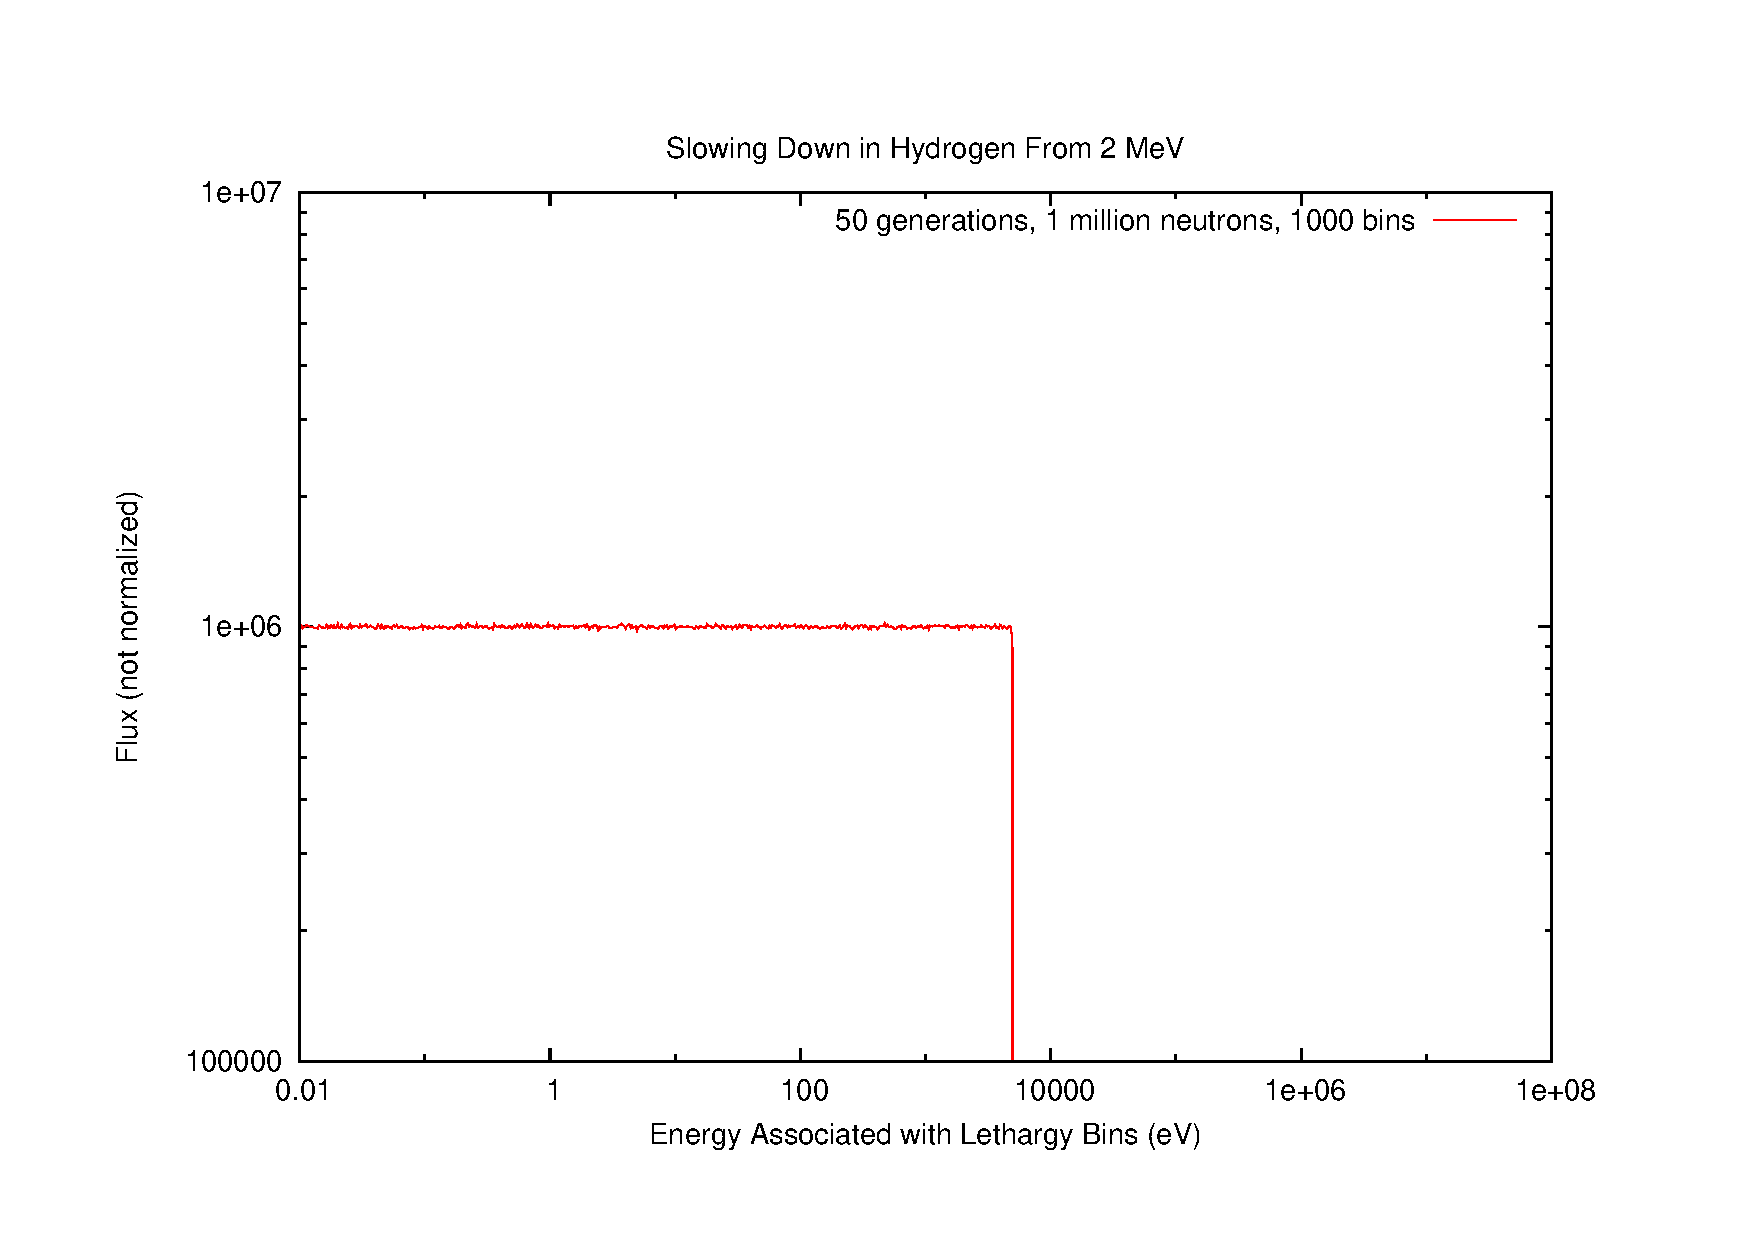
\includegraphics[width=0.3\textwidth]{images/sl-d/spec-1.uncrop.pdf} & asymptotic elastic scattering in hydrogen with source neutrons from 2 MeV \\ 
    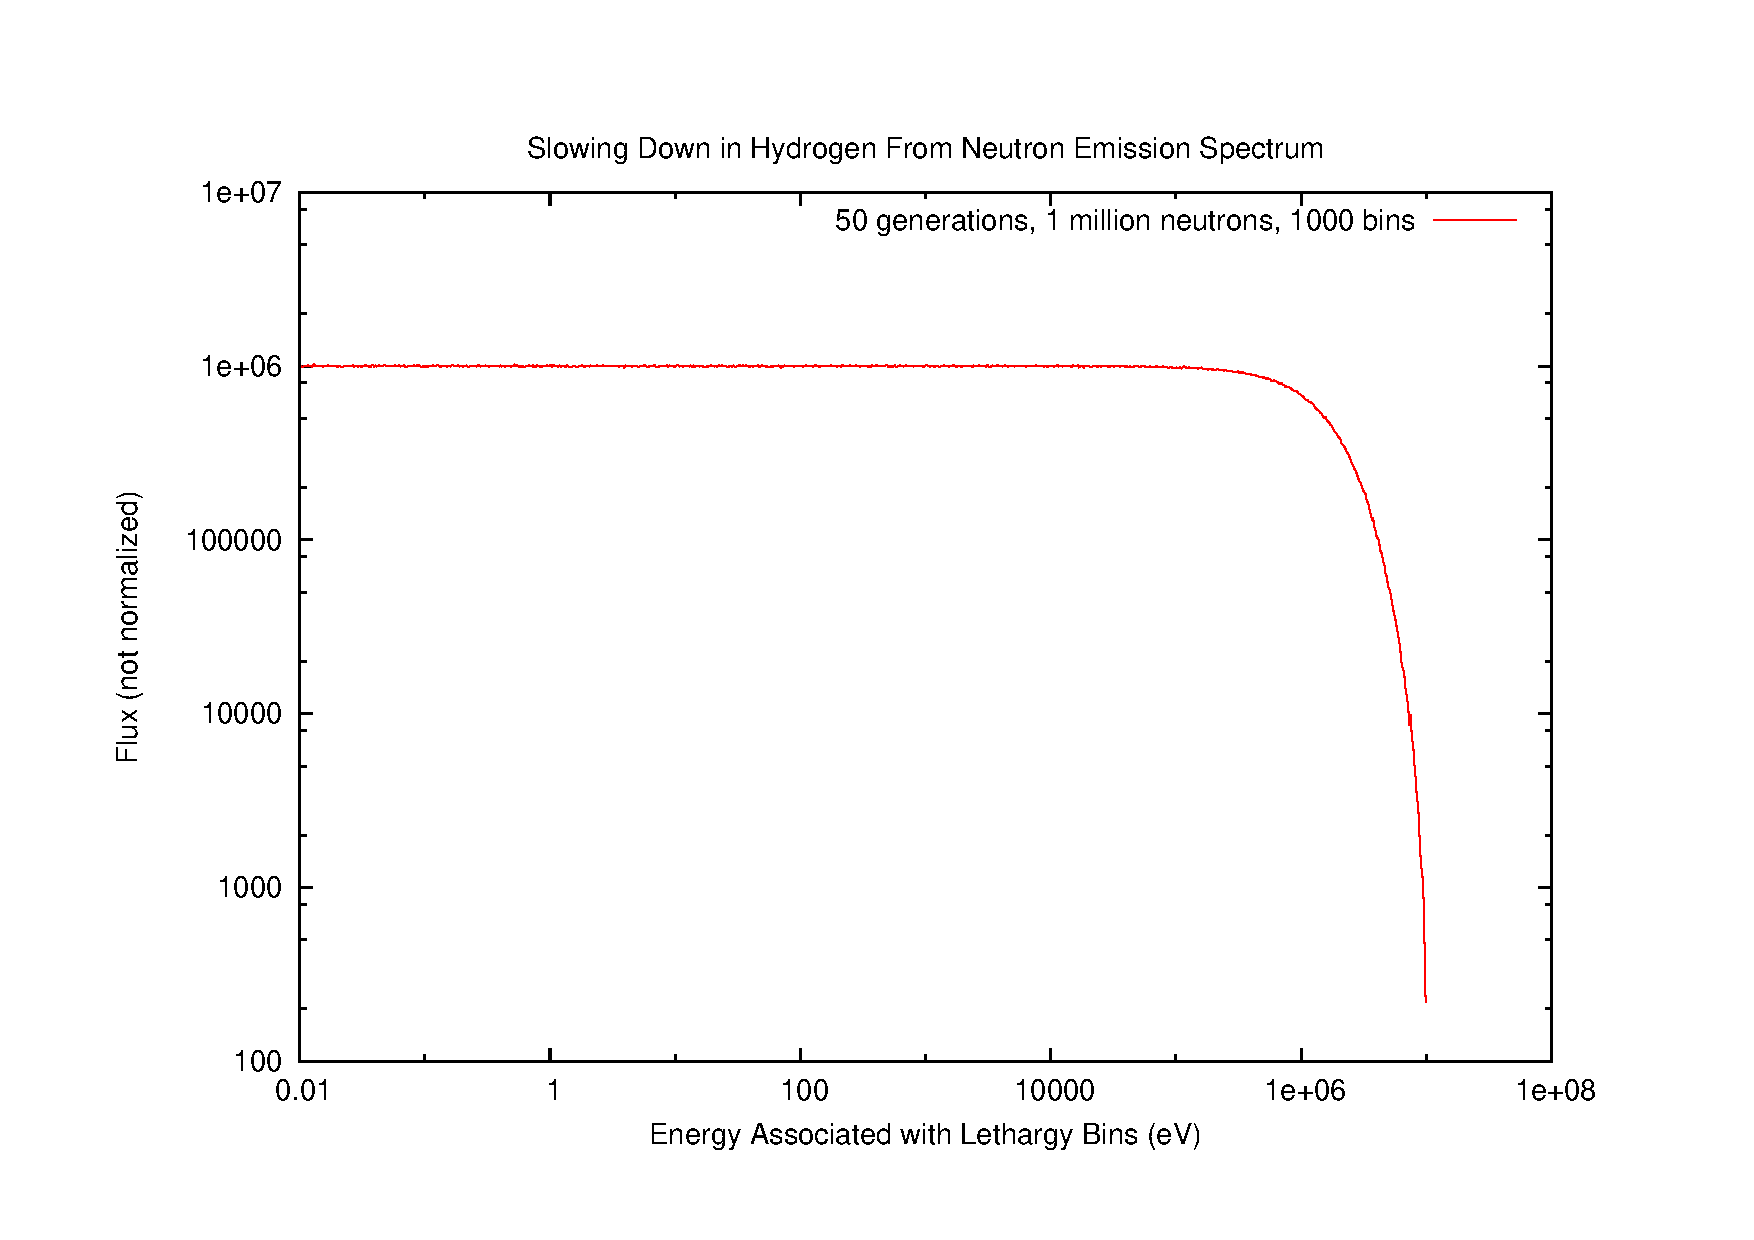
\includegraphics[width=0.3\textwidth]{images/sl-d/spec-2.uncrop.pdf} & replace source neutrons with neutron emission spectrum \\
    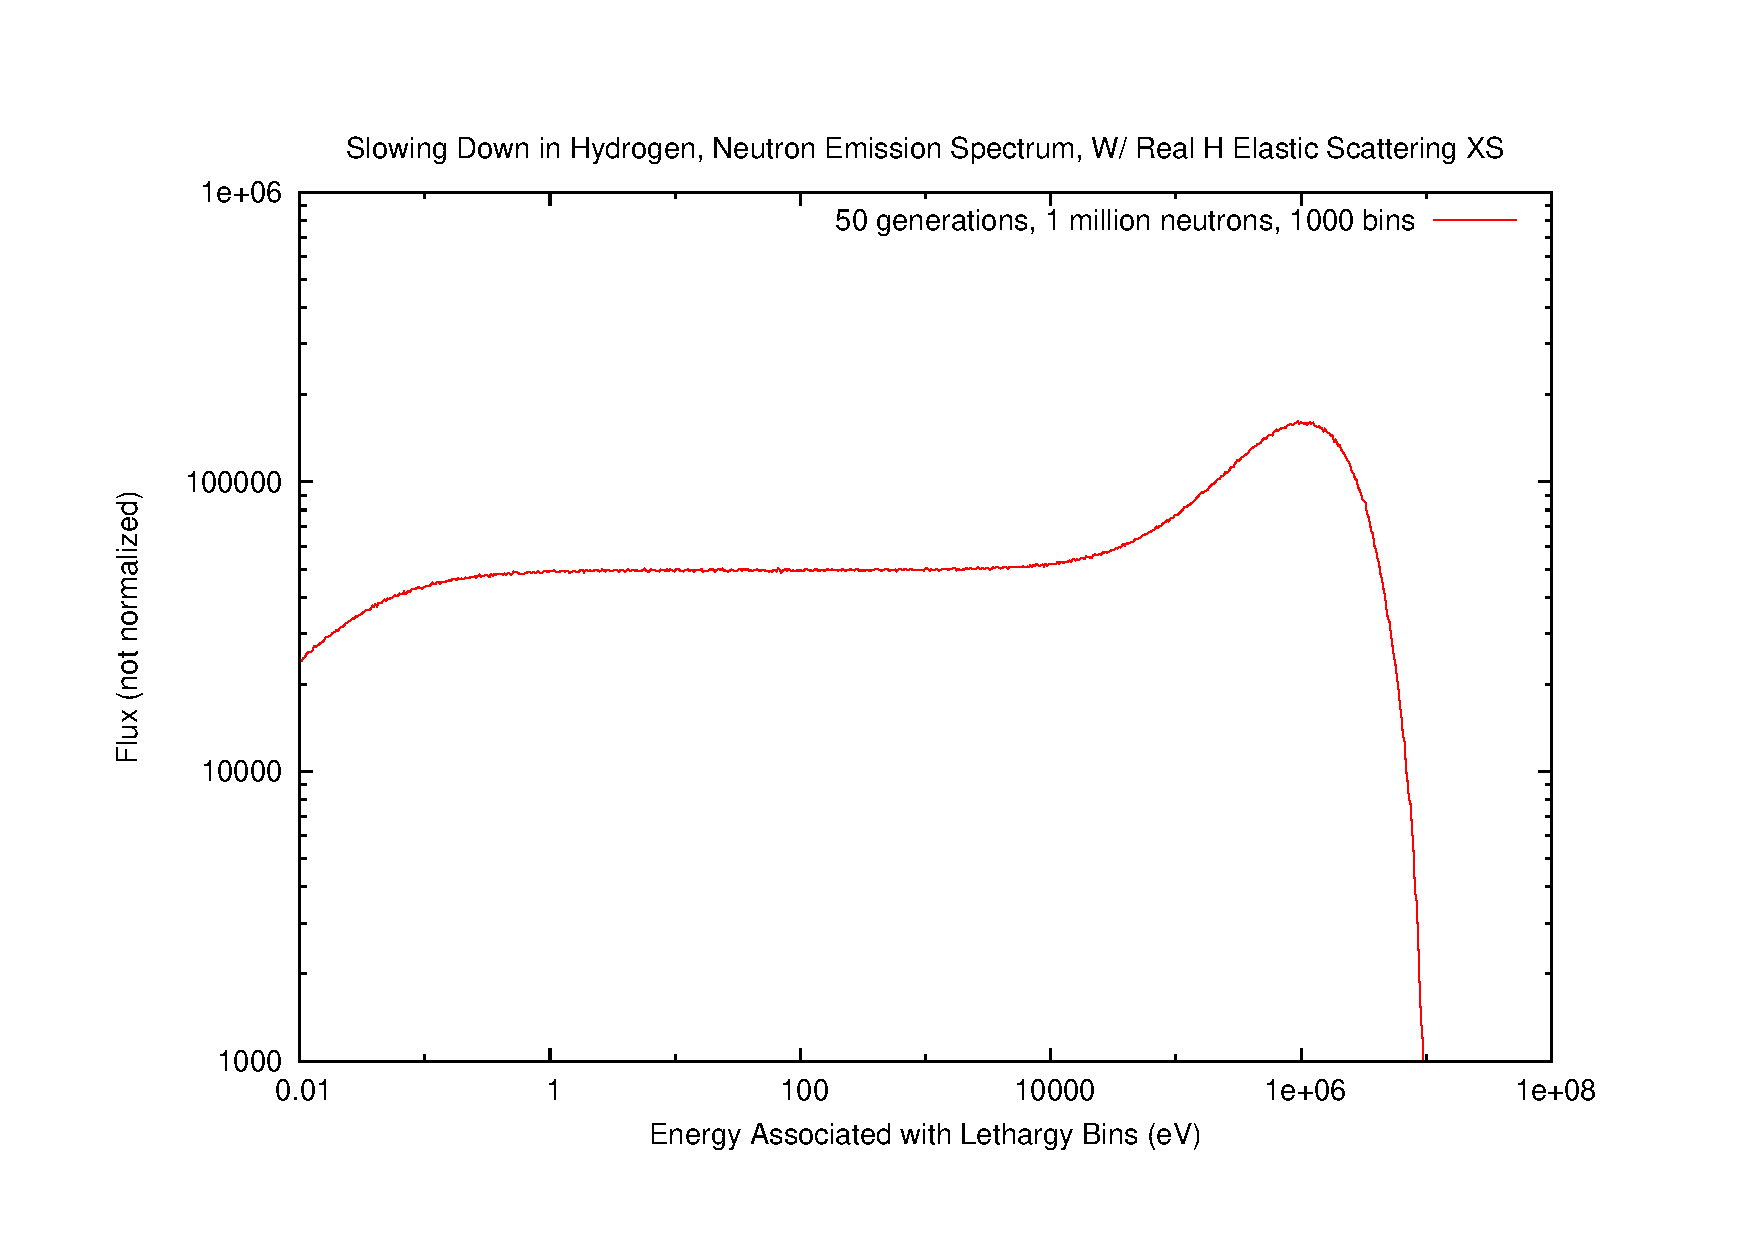
\includegraphics[width=0.3\textwidth]{images/sl-d/spec-3.uncrop.pdf} & add in real H elastic scattering xs (to divide the flux counter by) \\
    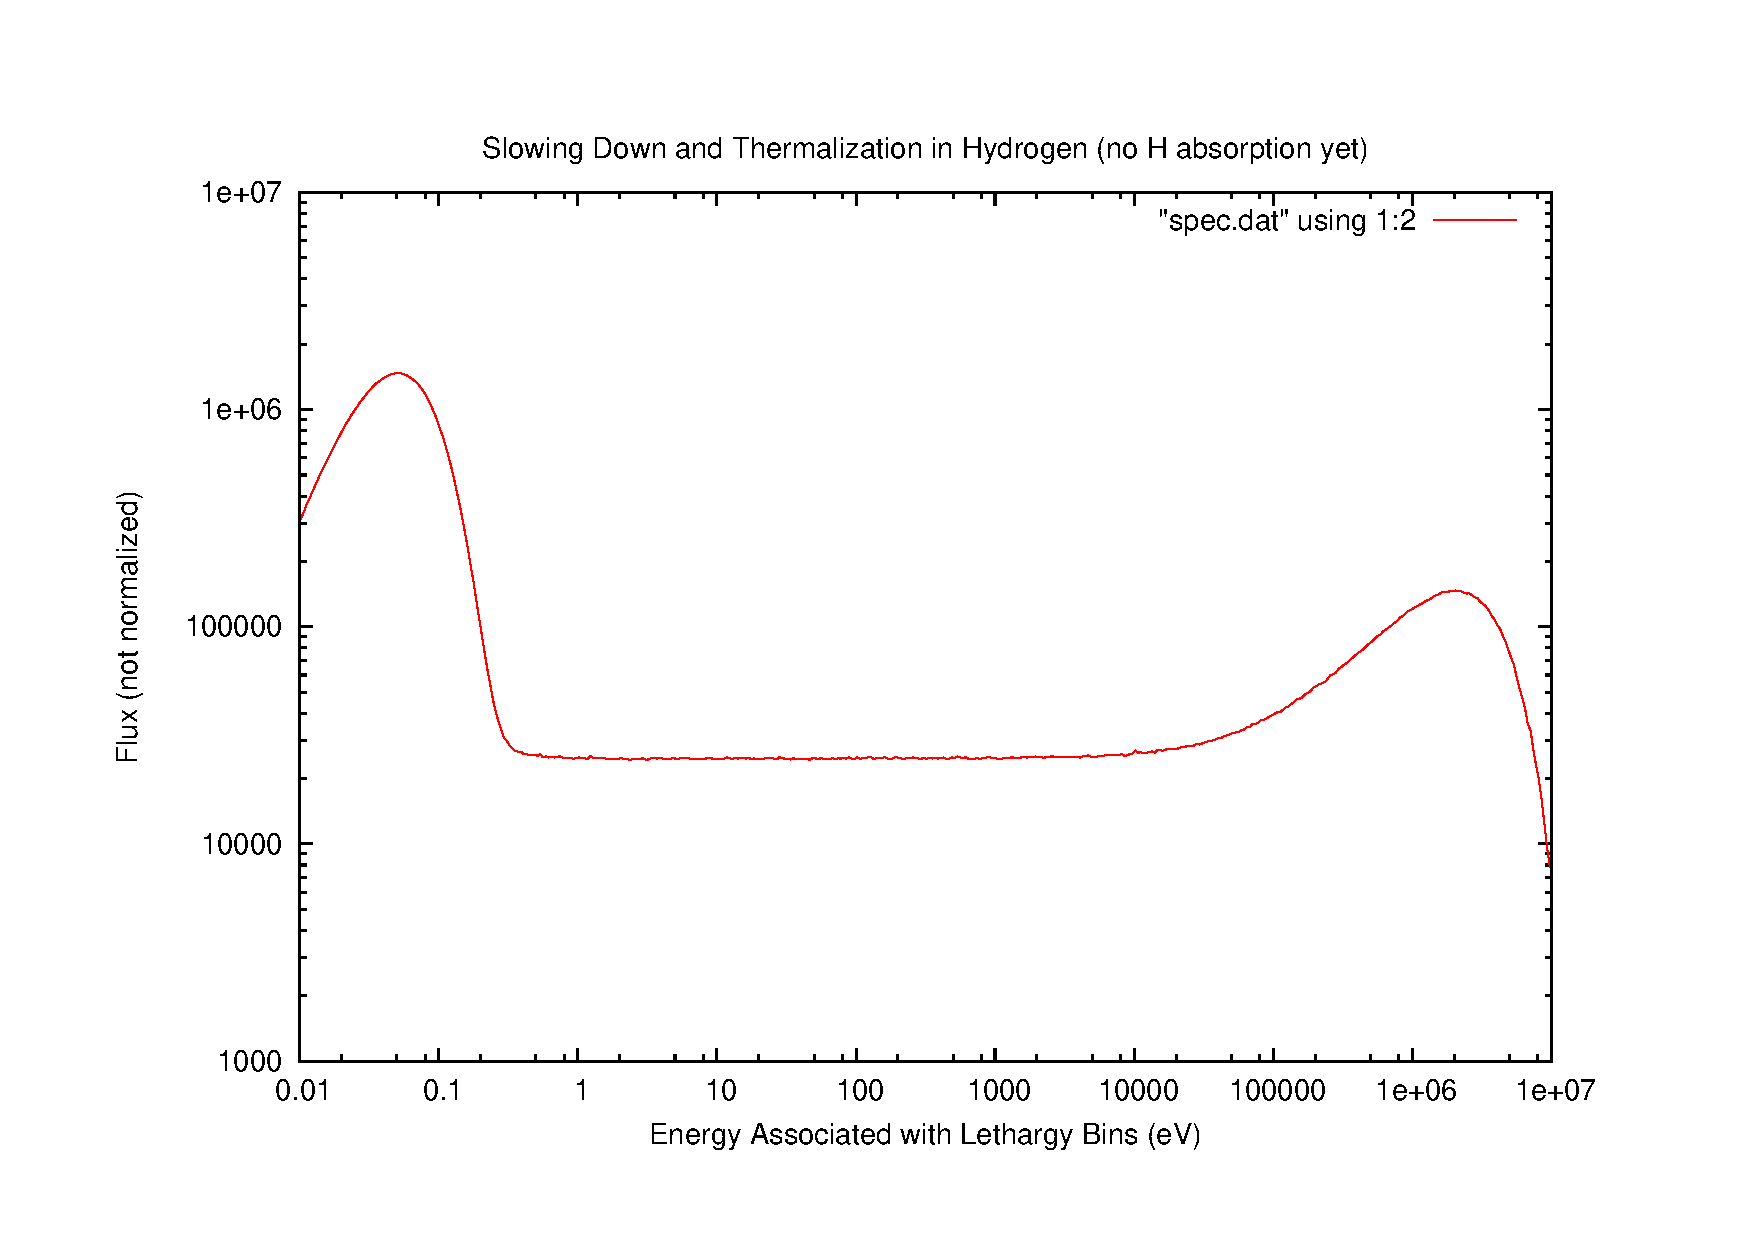
\includegraphics[width=0.3\textwidth]{images/sl-d/spec-4.uncrop.pdf} & add in thermalization in hydrogen ($<$ 4 eV, thermal scattering) \\
    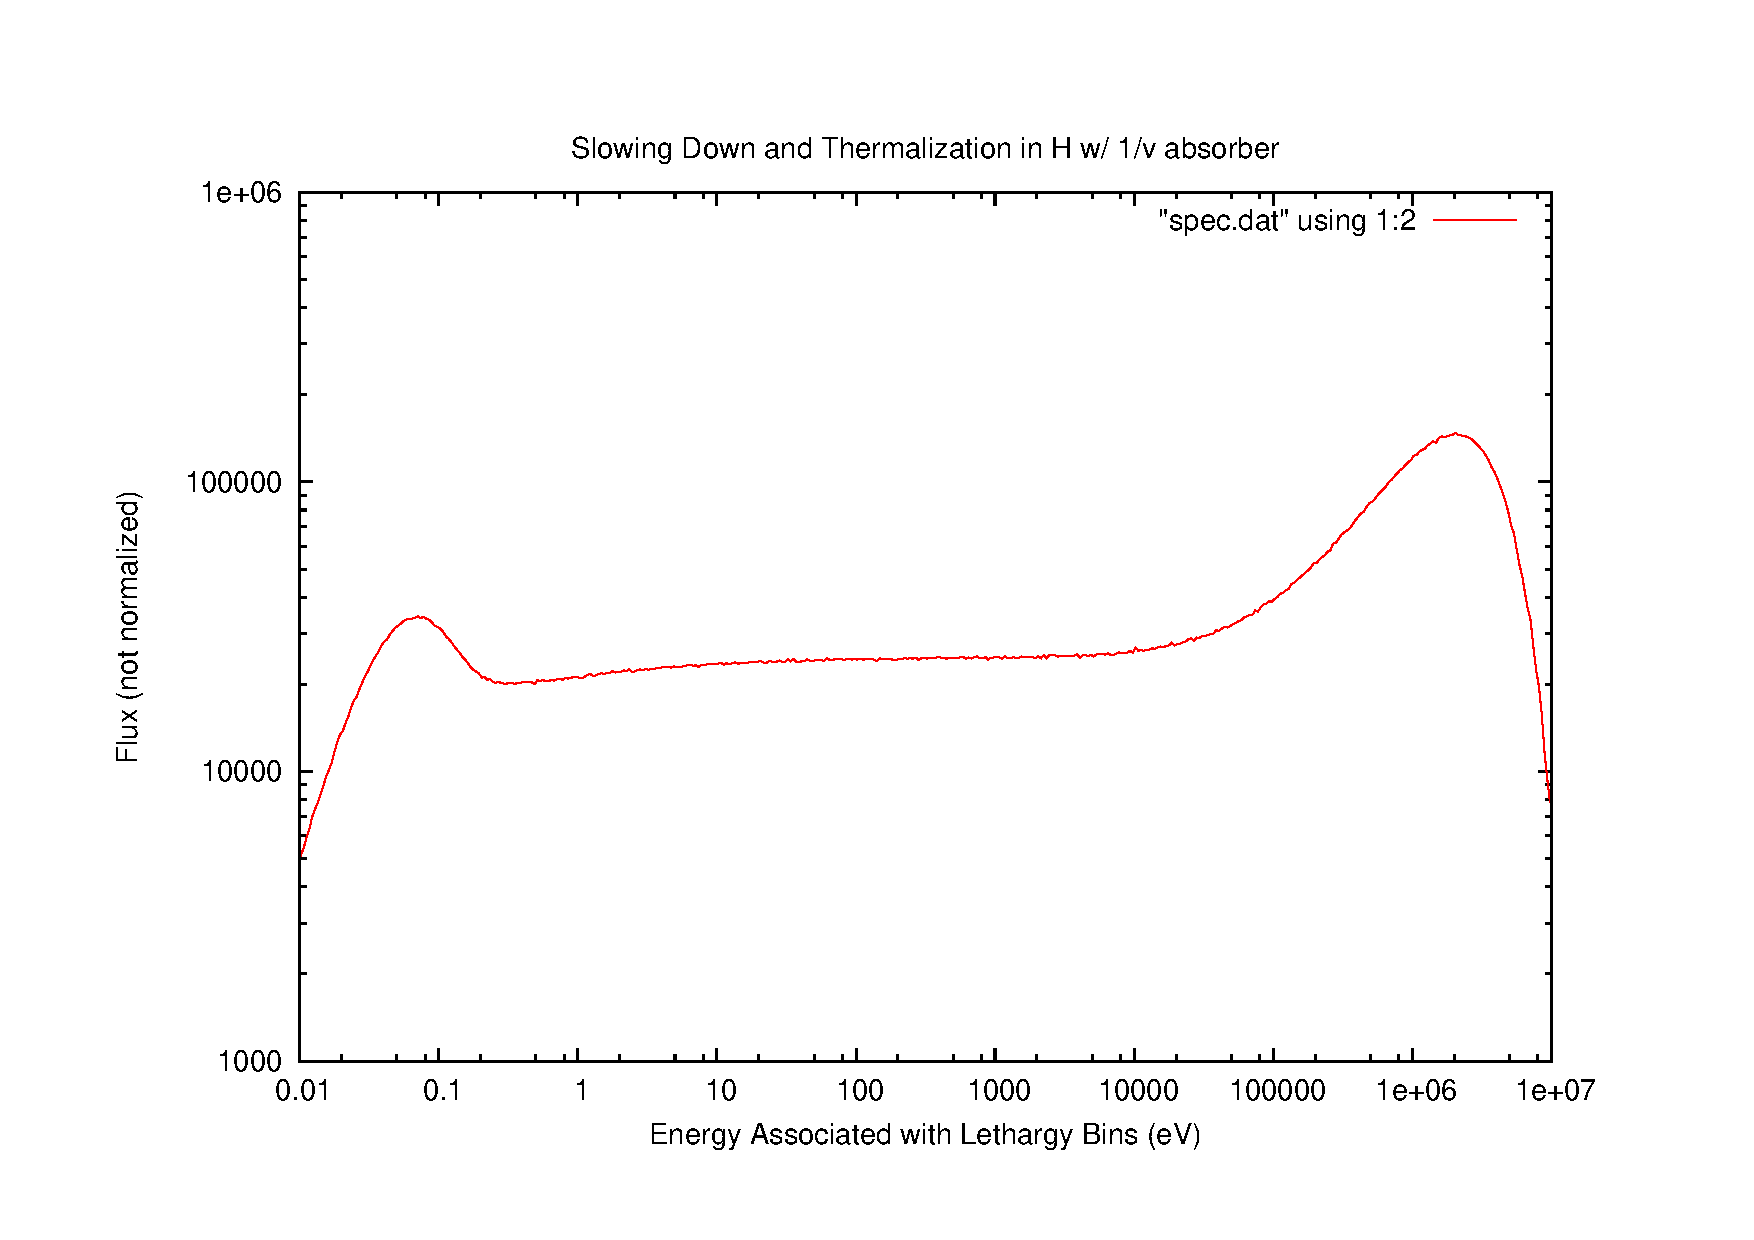
\includegraphics[width=0.3\textwidth]{images/sl-d/spec-5.uncrop.pdf} & add in 1/v H absorber (effective only in the thermal range) \\
    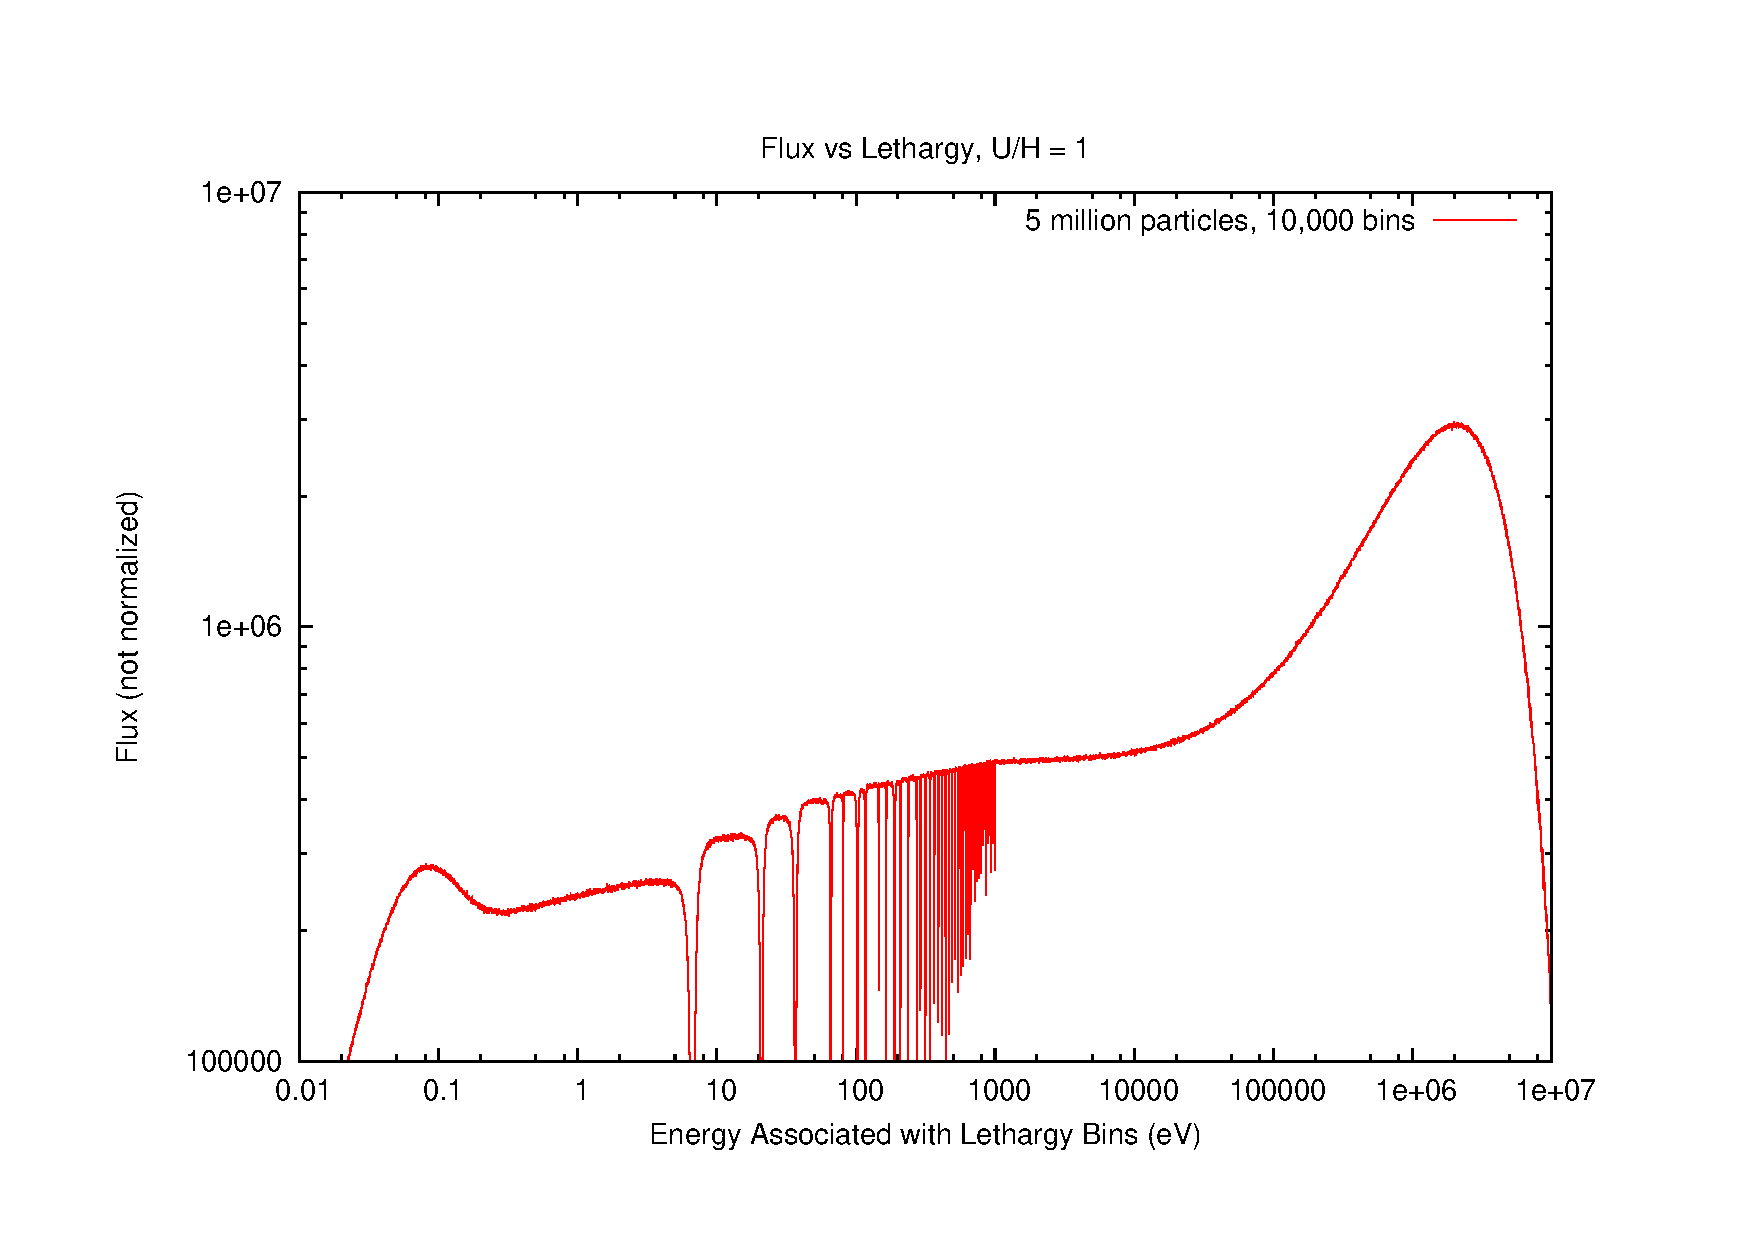
\includegraphics[width=0.3\textwidth]{images/sl-d/spec-7.uncrop.pdf} & add in U238 resonance absorption cross section \\
  \end{tabular}
  \caption{Physics and Their Corresponding Spectra in MC code} \label{plot-MC}
\end{table}

\topic{Concepts I got wrong in Exam 1}
\begin{enumerate}
\item $1/v$ cross section shape due to thermal motion. [2]
\item Thermal scattering kernel: notice for symmetry; know how to go from pdf to cdf etc. [1]
\item Resonance Integral: only include the resonance cross section, not the potential cross section. [2]
\item Infinite dilute implies that here is no neutrons being absorbed by the resonances. Recall that in HW2 when our U/H is small, the flux is not perturbed by U238 resonances at all, suggesting that the resonance escape probability is one. [1]
\item Calculate effective RI through $\RIeff = \int \sigma_r \phi \frac{1}{E} \dE.$ There is no integration of flux on the bottom (only introduced group xs's definition for the simulation's purpose). [2]
\item Calculate probabilities in 2 region setup. [3]
\item Monte Carlo tallies: U238 absorption rate can be estimated as $\Sum \frac{\Sigma_a}{\Sigma_t}$, the U238 absorption rate per atom is $\Sum \frac{\sigma_a}{\Sigma_t}$. [2]
\end{enumerate}
%%%%%%%%%%%%%%%%%%%%%%%%%%%% Exam 1 Review End %%%%%%%%%%%%%%%%%%%%%%%%%%%%%%%%%%%%%%%%%%



\end{document}
